\section{Sensors and state estimation}\label{sec:est}

The controllers of \cref{sec:control} use the full state
$\bm s = [x, \theta, \dot x, \dot\theta]^{\mathsf T}$. On the robot the state is
reconstructed from an inertial measurement unit (MPU-6050: three-axis
accelerometer and gyroscope) mounted on the body, and from the encoders of the
motors. This section gives the models of these sensors, the characteristics
measured on the MPU-6050, and the estimator.

\subsection{Sensor models}

\paragraph{Accelerometer.} The IMU is mounted on the body axis at a distance
$d = \SI{0.10}{m}$ from the axle. Its position and its two time derivatives are
\begin{align}
  \bm p_{\mathrm{imu}} &= \begin{bmatrix} x + d\sin\theta \\ d\cos\theta \end{bmatrix}, \qquad
  \dot{\bm p}_{\mathrm{imu}} = \begin{bmatrix} \dot x + d\cos\theta\,\dot\theta \\ -d\sin\theta\,\dot\theta \end{bmatrix}, \\
  \ddot{\bm p}_{\mathrm{imu}} &= \begin{bmatrix}
    \ddot x + d\cos\theta\,\ddot\theta - d\sin\theta\,\dot\theta^2 \\
    -d\sin\theta\,\ddot\theta - d\cos\theta\,\dot\theta^2 \end{bmatrix} .
\end{align}
An accelerometer measures the specific force, i.e.\ its acceleration minus the
gravitational acceleration $\bm g = [0, -g]^{\mathsf T}$:
\begin{equation}
  \bm f = \ddot{\bm p}_{\mathrm{imu}} - \bm g
  = \begin{bmatrix} \ddot p_x \\ \ddot p_z + g \end{bmatrix} ,
\end{equation}
expressed along the body axes
$\bm e_{\mathrm{up}} = [\sin\theta, \cos\theta]^{\mathsf T}$ (from the axle
towards the centre of mass) and
$\bm e_{\mathrm{fwd}} = [\cos\theta, -\sin\theta]^{\mathsf T}$:
\begin{equation}
  a_{\mathrm{fwd}} = \bm f\cdot\bm e_{\mathrm{fwd}} , \qquad
  a_{\mathrm{up}} = \bm f\cdot\bm e_{\mathrm{up}} .
\end{equation}
At rest $\bm f = [0, g]^{\mathsf T}$, so $a_{\mathrm{fwd}} = -g\sin\theta$ and
$a_{\mathrm{up}} = g\cos\theta$, and the tilt is
\begin{equation}
  \theta_{\mathrm{acc}} = \operatorname{atan2}\left(-a_{\mathrm{fwd}},\ a_{\mathrm{up}}\right) .
  \label{eq:acc-angle}
\end{equation}
When the robot accelerates, the terms in $\ddot x$, $\ddot\theta$ and
$\dot\theta^2$ also enter $\bm f$, and \cref{eq:acc-angle} no longer gives the
tilt. Gaussian noise is added to both components.

\paragraph{Gyroscope.} It measures $\dot\theta$ plus a constant bias $b$ and
Gaussian noise.

\paragraph{Encoders.} Each encoder is mounted on its motor, so it measures the
rotation of the wheel relative to the body, $\varphi - \theta$. With 11 pulses
per motor turn (assumed), the 21.3:1 gearbox and quadrature decoding, one wheel turn
gives $11 \times 21.3 \times 4 = 937$ counts; the count is the integer part of
$937\,(\varphi - \theta)/2\pi$. The position follows from the count and the
estimated tilt, $\hat x = r\,(\varphi_{\mathrm{rel}} + \hat\theta)$, and the velocity
from the difference of two consecutive positions, low-pass filtered:
\begin{equation}
  \hat{\dot x}_{k} = 0.8\,\hat{\dot x}_{k-1} + 0.2\,\frac{\hat x_k - \hat x_{k-1}}{\Delta t} .
\end{equation}

\subsection{Measured IMU characteristics}

The MPU-6050 was recorded at rest on a table for \SI{60}{s} at \SI{200}{Hz},
with its internal low-pass filter at \SI{44}{Hz}, ranges $\pm 8\,g$ and
$\pm\SI{500}{\degree/s}$ (\cref{tab:imu}; 11\,673 samples).

\begin{table}[h]
\centering
\caption{MPU-6050 at rest: mean and standard deviation of the readings.}
\label{tab:imu}
\begin{tabular}{@{}lccc@{}}
\toprule
 & $x$ & $y$ & $z$ \\
\midrule
Accelerometer, mean [\si{m/s^2}] & 0.181 & 0.266 & 10.015 \\
Accelerometer, std [\si{m/s^2}] & 0.014 & 0.014 & 0.020 \\
Gyroscope, mean [\si{\degree/s}] & $-1.59$ & $-1.50$ & $-0.06$ \\
Gyroscope, std [\si{\degree/s}] & 0.037 & 0.039 & 0.043 \\
\bottomrule
\end{tabular}
\end{table}

The magnitude of the mean acceleration is \SI{10.02}{m/s^2}, 2\% above $g$; a
scale error common to the two axes cancels in \cref{eq:acc-angle}. The gyroscope
means are its bias; they change by less than \SI{0.01}{\degree/s} between the
first and the last \SI{10}{s} of the recording. Subtracting the mean of the
first \SI{2}{s}, the angle obtained by integrating the gyroscope deviates by
\SI{1.1}{\degree} after \SI{60}{s}, i.e.\ a residual bias of about
\SI{0.02}{\degree/s}. The simulation uses an accelerometer noise of
\SI{0.015}{m/s^2}, a gyroscope noise of \SI{0.04}{\degree/s} and a gyroscope
bias of \SI{0.02}{\degree/s}.

\subsection{Complementary filter}

The two angle measurements have opposite defects: integrating the gyroscope is
accurate over short times but accumulates the bias; the accelerometer angle
does not drift but is disturbed by the accelerations of the robot. The filter
predicts the tilt with the gyroscope and corrects the prediction by a small
fraction towards the accelerometer angle at every step:
\begin{equation}
  \hat\theta_{k+1} = \alpha\left(\hat\theta_k + \omega_{g,k}\,\Delta t\right)
                     + (1 - \alpha)\,\theta_{\mathrm{acc},k} ,
  \qquad 0 < \alpha < 1 ,
  \label{eq:cf}
\end{equation}
where $\omega_g$ is the gyroscope reading. With $\alpha = 1$ the filter reduces
to the integration of the gyroscope, with $\alpha = 0$ to the accelerometer
angle. The rate estimate is the gyroscope reading, $\hat{\dot\theta} = \omega_g$.

\paragraph{Time constant.} Subtracting $\hat\theta_k$ from both sides of
\cref{eq:cf} and dividing by $\Delta t$,
\begin{equation}
  \frac{\hat\theta_{k+1} - \hat\theta_k}{\Delta t}
  = \alpha\,\omega_{g,k} + \frac{1 - \alpha}{\Delta t}\left(\theta_{\mathrm{acc},k} - \hat\theta_k\right)
  = \alpha\left[\omega_{g,k} + \frac{\theta_{\mathrm{acc},k} - \hat\theta_k}{T}\right],
  \qquad T = \frac{\alpha\,\Delta t}{1 - \alpha} .
\end{equation}
The estimate follows the gyroscope, and a difference from the accelerometer
angle is corrected with time constant $T$: variations faster than $T$ come from
the gyroscope, slower ones from the accelerometer.

\paragraph{Effect of the bias.} With the robot at rest at $\theta_0$, the
readings are $\omega_g = b$ and $\theta_{\mathrm{acc}} = \theta_0$. At steady
state $\hat\theta_{k+1} = \hat\theta_k = \hat\theta$, and \cref{eq:cf} gives
\begin{equation}
  \hat\theta = \alpha\hat\theta + \alpha b\,\Delta t + (1 - \alpha)\theta_0
  \quad\Rightarrow\quad
  \hat\theta - \theta_0 = \frac{\alpha\,\Delta t}{1 - \alpha}\,b = b\,T .
\end{equation}
The bias produces a constant error $bT$ instead of an error growing in time.

\paragraph{Choice of $\alpha$.} The LQR of \cref{sec:control}, with the motor
model, was run on the estimated state, from rest with $\theta_0 = 10^\circ$, for
\SI{10}{s}, with three different noise sequences per value of $\alpha$
(\cref{tab:alpha}; $\Delta t = \SI{5}{ms}$). The initial estimate is the true
tilt.

\begin{table}[h]
\centering
\caption{Closed loop on the estimated state for several $\alpha$ (mean over
three noise sequences).}
\label{tab:alpha}
\begin{tabular}{@{}cccccc@{}}
\toprule
$\alpha$ & $T$ [s] & Falls & $\hat\theta - \theta$ rms [deg] & $\hat\theta - \theta$ max [deg] & $|x|$ max, last \SI{2}{s} [cm] \\
\midrule
0.95  & 0.09 & 3/3 & --   & --   & --   \\
0.98  & 0.24 & 0/3 & 2.33 & 3.51 & 15.2 \\
0.99  & 0.49 & 0/3 & 0.68 & 1.53 & 2.6  \\
0.995 & 0.99 & 0/3 & 0.29 & 0.84 & 1.2  \\
0.998 & 2.49 & 0/3 & 0.12 & 0.39 & 1.5  \\
0.999 & 4.99 & 0/3 & 0.09 & 0.24 & 2.1  \\
\bottomrule
\end{tabular}
\end{table}

For small $\alpha$ the estimate follows the accelerometer angle, disturbed by
the accelerations produced by the controller itself: the estimation error
makes the robot oscillate, and for $\alpha = 0.95$ it falls. The error decreases
as $\alpha$ increases; with the measured bias, $bT$ is \SI{0.05}{\degree} for
$\alpha = 0.998$ and \SI{0.10}{\degree} for $\alpha = 0.999$. The value
$\alpha = 0.998$ ($T = \SI{2.5}{s}$) is used.

\subsection{Results}

\Cref{fig:est} compares, along the trajectory of the LQR with the true state
($\theta_0 = 10^\circ$, \SI{8}{s}), the error of three tilt estimates computed
from the same simulated readings: the accelerometer angle
\cref{eq:acc-angle} (rms \SI{0.90}{\degree}, maximum \SI{14.5}{\degree} during
the initial recovery), the integration of the gyroscope
(rms \SI{0.08}{\degree}, maximum \SI{0.14}{\degree}) and the complementary filter
(rms \SI{0.11}{\degree}, maximum \SI{0.37}{\degree}). Over \SI{8}{s} the
residual bias moves the integrated gyroscope by at most \SI{0.16}{\degree};
this error grows linearly with time, while the contribution of the bias to the
error of the filter is bounded by $bT$.

\begin{figure}[h]
\centering
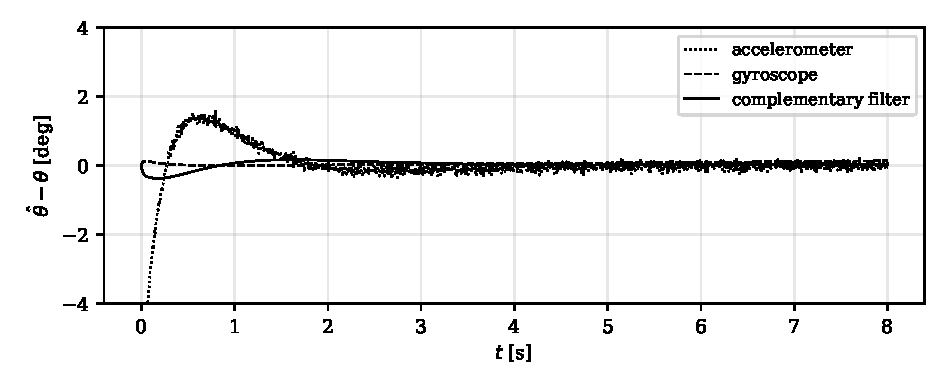
\includegraphics[width=\linewidth]{figures/estimation_error.pdf}
\caption{Error of three estimates of the tilt along the same trajectory (LQR
with the motor model, $\theta_0 = 10^\circ$), simulated sensors with the
measured noise and bias; complementary filter with $\alpha = 0.998$.}
\label{fig:est}
\end{figure}

With the LQR running on the estimated state (complementary filter and encoder
odometry), the robot is upright after \SI{8}{s} ($\theta = \SI{0.01}{\degree}$)
at $x = \SI{-1.3}{cm}$ from the starting point.
